\documentclass[12pt]{article}
%% arXiv paper template by Flip Tanedo


%%%%%%%%%%%%%%%%%%%%%%%%%%%%%
%%%  THE USUAL PACKAGES  %%%%
%%%%%%%%%%%%%%%%%%%%%%%%%%%%%

\usepackage{amsmath}         % \
\usepackage{amssymb}         %  | AMS Packages for math
\usepackage{amsfonts}        % /
\usepackage{graphicx}        % Graphics
 

%%%%%%%%%%%%%%%%%%%%%%%%%%%%%%%%%
%%%  UNUSUAL PACKAGES        %%%%
%%%  Uncomment as necessary. %%%%
%%%%%%%%%%%%%%%%%%%%%%%%%%%%%%%%%

\usepackage{lipsum}        % block of text (formatting test)
%\usepackage{color}         % \color{...}, colored text
%\usepackage{slashed}       % \slashed{k}
%\usepackage{framed}        % boxed remarks
%\usepackage{subcaption}    % subfigures; subfig depreciated
%\usepackage{mathrsfs}      % Weinberg-esque letters
%\usepackage{paralist}      % compactitem
%\usepackage{multirow}      % multiple row elements in a table
%\usepackage{cite}          % grouping citations (incompatible with collref)
%\usepackage{booktabs}      % tables
%\usepackage{nicefrac}      % fractions in tables,
%\usepackage{youngtab}	    % Young Tableaux
%\usepackage{arydshln} 	    % dashed lines in arrays and tables
%\usepackage{appendix}      % subappendices
%\usepackage{pifont}        % check marks
%\usepackage{bbm}           % \mathbbm{1} incompatible with XeLaTeX 


%%%%%%%%%%%%%%%%%%%%%%%%%%%%%%%%%%%%%%%%%%%
%%%  FLIP'S CUSTOM PACKAGES            %%%%
%%%  These are in separate .sty files  %%%%
%%%%%%%%%%%%%%%%%%%%%%%%%%%%%%%%%%%%%%%%%%%

\usepackage{flip-acronyms} % HEP acronyms in small caps, e.g. \GeV
\usepackage{tikzfeynman}   % Flip's Feynman Diagrams


%%%%%%%%%%%%%%%%%%%%%%%%%%%%%%%%%%%%%%%%%%%%%%%
%%%  PAGE FORMATTING and (RE)NEW COMMANDS  %%%%
%%%%%%%%%%%%%%%%%%%%%%%%%%%%%%%%%%%%%%%%%%%%%%%


\usepackage[margin=2cm]{geometry}   % reasonable margins
\graphicspath{{figures/}}	        % set directory for figures
\numberwithin{equation}{section}    % set equation numbering
\renewcommand{\tilde}{\widetilde}   % tilde over characters
\renewcommand{\vec}[1]{\mathbf{#1}} % vectors are boldface


\newcommand{\dbar}{d\mkern-6mu\mathchar'26}    % for d/2pi
\newcommand{\ket}[1]{\left|#1\right\rangle}    % <#1|
\newcommand{\bra}[1]{\left\langle#1\right|}    % |#1>
\newcommand{\Xmark}{\text{\sffamily X}}        % cross out


% Commands for temporary comments
\newcommand{\comment}[2]{\textcolor{red}{[\textbf{#1} #2]}}
\newcommand{\flip}[1]{{\tt \color{red} [Flip: {#1}]}}
\newcommand{\email}[1]{\href{mailto:#1}{#1}}


\newenvironment{institutions}[1][2em]{\begin{list}{}{\setlength\leftmargin{#1}\setlength\rightmargin{#1}}\item[]}{\end{list}}


%%%%%%%%%%%%%%%%%%%%%%%%%%%%%%%%%%%%%%%%%%%%%%
%%%  TIKZ COMMANDS FOR EXTERNAL DIAGRAMS  %%%%
%%%  requires -shell-escape               %%%%
%%%%%%%%%%%%%%%%%%%%%%%%%%%%%%%%%%%%%%%%%%%%%%

%\usetikzlibrary{external}
%\tikzexternalize[prefix=tikz/] % folder for external pdfs



%%%%%%%%%%%%%%%%%%%
%%%  HYPERREF  %%%%
%%%%%%%%%%%%%%%%%%%

% This package has to be at the end; can lead to conflicts
\usepackage[
	colorlinks=true,
	citecolor=black,
	linkcolor=black,
	urlcolor=blue,
	hypertexnames=false]{hyperref}



%%%%%%%%%%%%%%%%%%%%%
%%%  TITLE DATA  %%%%
%%%%%%%%%%%%%%%%%%%%%


\begin{document}

\thispagestyle{empty}
\begin{center}

    {\huge \textbf{Sample Feynman Diagrams in TikZ} \\
    \large \textsc{Vol.~V: Common Processes} }

    \vskip .7cm

    { \bf Flip Tanedo } 
    \\ \vspace{-.2em}
    { \tt
    \footnotesize
    \email{flip.tanedo@uci.edu} 
    }
	
    \vspace{-.2cm}

    \begin{institutions}[2.25cm]
    \footnotesize
	\vspace*{0.05cm}
	{\it 
	    Department of Physics \& Astronomy, 
	    University of California, 
	    Irvine, \textsc{ca} 92697
	    }   
    \end{institutions}

\end{center}



%%%%%%%%%%%%%%%%%%%%%
%%%  ABSTRACT    %%%%
%%%%%%%%%%%%%%%%%%%%%

\begin{abstract}
\noindent This is collection of useful sample Feynman diagrams and pieces typeset in TikZ. See Volume I for background information.
\end{abstract}




%%%%%%%%%%%%%%%%%%%%%
%%%  THE MEAT    %%%%
%%%%%%%%%%%%%%%%%%%%%

% Use \input if you have separate files.
% \include is `smarter' (creates separate aux files for each tex file) 
% and hence more efficient, but it automatically puts a page break
% between included files. Input doesn't do this.

\section{Higgs Production}


\begin{tikzpicture}[line width=1.5 pt]
	\draw[gluon] (120:1) -- (120:2);
	\draw[scalarnoarrow] (0:1) -- (0:2);
	\draw[gluon] (240:1) -- (240:2);
	\draw[fermion] (120:1) -- (240:1);
	\draw[fermion] (240:1) -- (0:1);
	\draw[fermion] (0:1) -- (120:1);
 \end{tikzpicture}

\vspace{1em}

\begin{tikzpicture}[line width=1.5 pt]
	\draw[gluon] (-.5,0) -- (1,0);
	\draw[gluon] (-.5,2) -- (1,2);
	\draw[fermionbar] (1,2) -- (1,1);
	\draw[fermionbar] (1,1) -- (1,0);
	\draw[scalarnoarrow] (1,1) -- (2.5,1);
	\draw[fermionbar] (1,0) -- (2.5,0);
	\draw[fermion] (1,2) -- (2.5,2);
 \end{tikzpicture}



\vspace{1em}

\begin{tikzpicture}[line width=1.5 pt]
	\draw[fermion] (-.5,0) -- (1,0);
	\draw[fermion] (-.5,2) -- (1,2);
	\draw[vector] (1,2) -- (1,1);
	\draw[vector] (1,1) -- (1,0);
	\draw[scalarnoarrow] (1,1) -- (2.5,1);
	\draw[fermion] (1,0) -- (2.5,0);
	\draw[fermion] (1,2) -- (2.5,2);
 \end{tikzpicture}

\vspace{1em}

\vspace{1em}
\begin{tikzpicture}[line width=1.5 pt, scale=1.3]
	\draw[fermionbar] (-140:1)--(0,0);
	\draw[fermion] (140:1)--(0,0);
	\draw[vector] (0:1)--(0,0);
	% \node at (-140:1.2) {$e$};
	% \node at (140:1.2) {$e$};
	% \node at (.5,.3) {$Z$};	
\begin{scope}[shift={(1,0)}]
	\draw[vector] (-40:1)--(0,0);
	\draw[scalarnoarrow] (40:1)--(0,0);
	% \node at (-40:1.2) {$\mu$};
	% \node at (40:1.2) {$\mu$};	
\end{scope}
\end{tikzpicture}




\section{Coleman--Weinberg}

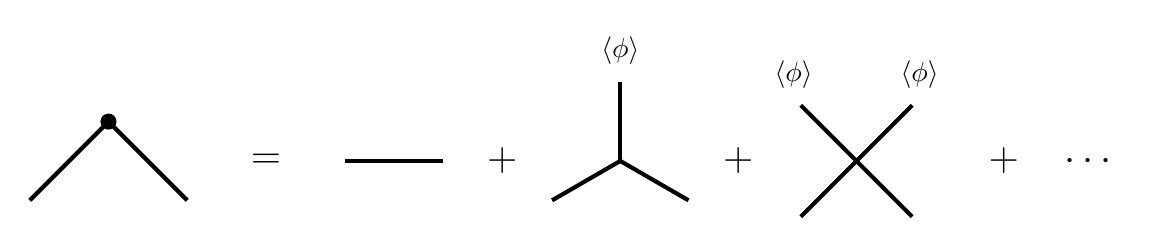
\begin{tikzpicture}[line width=1.5 pt]
	\draw (-1,-.5) -- (0,.5) -- (1,-.5);
	\draw[fill=black] (0,.5) circle (.075cm);
	\node at (2,0) {\Large=};
	\draw (3,0) -- (4.25,0);
	\node at (5,0) {\Large+};
	\draw (-30:1)+(6.5,0) -- (6.5,0);
	\draw (90:1)+(6.5,0) -- (6.5,0);
	\draw (210:1)+(6.5,0) -- (6.5,0);
	\node at (6.5,1.4) {$\langle \phi\rangle$};
	\node at (8,0) {\Large+};
	\draw (45:1)+(9.5,0) -- (9.5,0);
	\draw (135:1)+(9.5,0) -- (9.5,0);
	\draw (225:1)+(9.5,0) -- (9.5,0);
	\draw (315:1)+(9.5,0) -- (9.5,0);
	\node at (8.7,1.1) {$\langle \phi\rangle$};
	\node at (10.3,1.1) {$\langle \phi\rangle$};
	\node at (12,0) {\Large$+\hspace{.5cm}\cdots$};
 \end{tikzpicture}

\vspace{1em}

\begin{tikzpicture}[line width=1.5 pt]
	\draw (-1,-.5) -- (0,.5) -- (1,-.5);
	\draw[fill=black] (0,.5) circle (.075cm);
	\node at (2,0) {\Large=};
	\draw (3,0) -- (4.25,0);
	\node at (5,0) {\Large+};
	\draw (-30:1)+(6.5,0) -- (6.5,0);
	\draw (90:1)+(6.5,0) -- (6.5,0);
	\draw (210:1)+(6.5,0) -- (6.5,0);
	% \node at (6.5,1.4) {$\langle \phi\rangle$};
	\node at (8,0) {\Large+};
	\draw (45:1)+(9.5,0) -- (9.5,0);
	\draw (135:1)+(9.5,0) -- (9.5,0);
	\draw (225:1)+(9.5,0) -- (9.5,0);
	\draw (315:1)+(9.5,0) -- (9.5,0);
	% \node at (8.7,1.1) {$\langle \phi\rangle$};
	% \node at (10.3,1.1) {$\langle \phi\rangle$};
	\node at (12,0) {\Large$+\hspace{.5cm}\cdots$};
	\begin{scope}[shift={(6.5,1)},scale=.7] % Mass Insertion
		\clip (0,0) circle (.25);
		\draw[fermionnoarrow] (-1,1) -- (1,-1);
		\draw[fermionnoarrow] (1,1) -- (-1,-1);
	\end{scope}	
	%
	\begin{scope}[shift={(9.5,0)}]
	\begin{scope}[shift={(45:1)},scale=.7,rotate=45] % Mass Insertion
		\clip (0,0) circle (.25);
		\draw[fermionnoarrow] (-1,1) -- (1,-1);
		\draw[fermionnoarrow] (1,1) -- (-1,-1);
	\end{scope}	
	\end{scope}
	%
	\begin{scope}[shift={(9.5,0)}]
	\begin{scope}[shift={(135:1)},scale=.7,rotate=45] % Mass Insertion
		\clip (0,0) circle (.25);
		\draw[fermionnoarrow] (-1,1) -- (1,-1);
		\draw[fermionnoarrow] (1,1) -- (-1,-1);
	\end{scope}	
	\end{scope}
 \end{tikzpicture}



\section{Meson confinement}

	\begin{tikzpicture}[line width=1.5 pt, scale=1.3]
		\draw[fermion] (-1,0) -- (0,0);
		\draw[fermion] (0,0) -- (0,-1);
		\draw[fermion] (0,-1) -- (-1,-1);
		\draw[gluon] (0,0) -- (.5,0);
		\draw[gluon] (.5,0) -- (1,0);
		\draw[gluon] (.5,0) arc (180:270:.5);
		\draw[gluon] (0,-1) -- (1,-1);
		\draw[fermion] (2,-1) -- (1,-1);
		\draw[fermion] (1,-1) -- (1,-.5);
		\draw[fermion] (1,-.5) -- (1,0);
		\draw[fermion] (1,0) -- (1.5,0);
		\draw[fermion] (1.5,0) -- (2,0);
		\draw[fermion] (2,0) -- (2.5,0);
		\draw[fermion] (2.5,0) -- (3.5,0);
		\draw[gluon] (1.5,0) arc (180:0:.5);
		\draw[gluon] (2,0) -- (2,-.5);
		\draw[gluon] (2,-.5) -- (2,-1);
		\draw[gluon] (2,-.5) arc (90:0:.5);
		\draw[fermion] (3.5,-1) -- (2.5,-1);
		\draw[fermion] (2.5,-1) -- (2,-1);
	\end{tikzpicture}



\section{SUSY Cascade}
	
	
\begin{tikzpicture}[line width=1.5 pt]
	\draw[vector] (90:2) -- (45:2);
	\draw[fermionnoarrow] (90:2) -- (45:2);
	\draw[scalar] (45:2) -- (0:2);
	\draw[scalar] (-1.5,2) -- (0,2);
	\draw[vector] (2,0) -- (2,-1.5);
	\draw[fermionnoarrow] (2,0) -- (2,-1.5);
	%
	\draw[fermion] (90:2) -- (90:3.5);
	\draw[fermion] (45:2) -- (45:3.5);
	\draw[fermion] (0:2) -- (0:3.5);
\end{tikzpicture}




\section{Flavor}

\begin{tikzpicture}[line width=1.5 pt, scale=1.3]
	\everymath{\displaystyle}
%
	\node[draw,circle] (id1) at (0,1.7em) {$d$};
	\node[draw,circle] (id2) at (0,0em) {$u$};
	\node[draw,circle] (iu1) at (0,-1.7em) {$d$};
%
	\draw[dashed, black!30] (0,0) ellipse (1.8em and 3em); 	
%
	\node[draw,circle] (od1) at (8em,1.7em) {$d$};
	\node[draw,circle] (ou1) at (8em,0em) {$u$};
	\node[draw,circle] (ou2) at (8em,-1.7em) {$u$};
%
	\draw[dashed, black!30] (8em,0) ellipse (1.8em and 3em);
% 	
	\draw[fermion] (id1) -- (od1);
	\draw[fermion] (id2) -- (ou1);
	\draw[fermion] (iu1) -- (3em,-1.7em);
	\draw[fermion] (3em,-1.7em) -- (ou2);
   	\draw[snake=snake, line before snake=.5em] (3em,-1.7em) -- (5em, -4.5em); 
	\draw[fermion] (5em, -4.5em) -- (8em, -4em);
	\draw[fermionbar] (5em, -4.5em) -- (8em, -5.5em);
	% NOTE: snake = snake is important
	\node at (3em,-4em) {$W^+$};
	\node at (8.6em,-4em) {$\nu_e$};
	\node at (8.5em,-5.5em) {$e$};
\end{tikzpicture}


\vspace{1em}

\begin{center}
	\begin{tikzpicture}[line width=1.5 pt, scale=1.3]
		\draw[fermion] (15:1.5)--(0,0);
		\draw[fermionbar] (180:1)--(0,0);
		\draw[vector] (-40:1)--(0,0);
		\node at (15:1.7) {$c$};
		\node at (180:1.2) {$b$};
		% \node at (0.2,-.5) {$W$};
		\coordinate (uin) at (-1,-.3);
		\coordinate (umid) at (-80:.5);
	% \begin{scope}[shift={(0,.3)}]
	% 	\draw[fermion] (180:1) to [out=0,in=220] (40:1); 
	% 	\node at (40:1.4) {$d$};
	% 	\node at (180:1.2) {$d$};
	% \end{scope}
	\begin{scope}[shift={(-40:1)}]
		\draw[fermion] (-20:1)--(0,0);
		\draw[fermionbar] (40:1)--(0,0);
		\node at (40:1.2) {$u$};
		\node at (-20:1.2) {$s$};
		\coordinate (uend) at (-40:1.2);
		\node at (-40:1.4) {$u$};
	\end{scope}
	\draw[fermion] (uin) to [out=0, in=140] (umid) to [out=-35, in=160] (uend);
	\node at (-1.2,-.3) {$u$};
	\draw [gray,decorate,decoration={brace,amplitude=5pt},xshift=-4pt]
	   (-1.2,-.5)  -- (-1.2,.2) 
	   node [black,midway,left=4pt,xshift=-2pt] {$B^+$};
	\draw [gray,decorate,decoration={brace,amplitude=5pt},xshift=-4pt]
	   (2,.6)  -- (2,-.1) 
	   node [black,midway,right=4pt] {$\bar{D}$};
	\draw [gray,decorate,decoration={brace,amplitude=5pt},xshift=-4pt]
	   (2.2,-.8)  -- (2.2,-1.7) 
	   node [black,midway,right=4pt] {$K^+$};
	\end{tikzpicture}
	%
	%
	\qquad\qquad
	%
	%
	\begin{tikzpicture}[line width=1.5 pt, scale=1.3]
		\draw[fermion] (15:1.5)--(0,0);
		\draw[fermionbar] (180:1)--(0,0);
		\draw[vector] (-40:1)--(0,0);
		\node at (15:1.7) {$u$};
		\node at (180:1.2) {$b$};
		% \node at (0.2,-.5) {$W$};
		\coordinate (uin) at (-1,-.3);
		\coordinate (umid) at (-80:.5);
	% \begin{scope}[shift={(0,.3)}]
	% 	\draw[fermion] (180:1) to [out=0,in=220] (40:1); 
	% 	\node at (40:1.4) {$d$};
	% 	\node at (180:1.2) {$d$};
	% \end{scope}
	\begin{scope}[shift={(-40:1)}]
		\draw[fermion] (-20:1)--(0,0);
		\draw[fermionbar] (40:1)--(0,0);
		\node at (40:1.2) {$c$};
		\node at (-20:1.2) {$s$};
		\coordinate (uend) at (-40:1.2);
		\node at (-40:1.4) {$u$};
	\end{scope}
	\draw[fermion] (uin) to [out=0, in=140] (umid) to [out=-35, in=160] (uend);
	\node at (-1.2,-.3) {$u$};
	\draw [gray,decorate,decoration={brace,amplitude=5pt},xshift=-4pt]
	   (-1.2,-.5)  -- (-1.2,.2) 
	   node [black,midway,left=4pt,xshift=-2pt] {$B^+$};
	\draw [gray,decorate,decoration={brace,amplitude=5pt},xshift=-4pt]
	   (2,.6)  -- (2,-.1) 
	   node [black,midway,right=4pt] {$D$};
	\draw [gray,decorate,decoration={brace,amplitude=5pt},xshift=-4pt]
	   (2.2,-.8)  -- (2.2,-1.7) 
	   node [black,midway,right=4pt] {$K^+$};
	\end{tikzpicture}
\end{center}

\vspace{1em}

\begin{center}
	\begin{tikzpicture}[line width=1.5 pt, scale=1.3]
		\draw[fermion] (40:1.2)--(0,0);
		\draw[fermionbar] (180:1)--(0,0);
		\draw[vector] (-40:1)--(0,0);
		\node at (40:1.4) {$u$};
		\node at (180:1.2) {$b$};
		\node at (0.2,-.5) {$W$};
	\begin{scope}[shift={(0,.3)}]
		\draw[fermion] (180:1) to [out=0,in=220] (40:1); %****	
		\node at (40:1.4) {$d$};
		\node at (180:1.2) {$d$};
	\end{scope}
	\begin{scope}[shift={(-40:1)}]
		\draw[fermion] (-20:1)--(0,0);
		\draw[fermionbar] (20:1)--(0,0);
		\node at (-20:1.2) {$s$};
		\node at (20:1.2) {$u$};
	\end{scope}
	\end{tikzpicture}
\end{center}



\section{Graviton lines}


\begin{center}
\begin{tikzpicture}[line width=1.5 pt]
\draw[vector, line width=.75] (0,0) -- (2,0);
\draw[vector, line width=.75] (0,-.1) -- (2,-.1);
\draw[fermion] (-1,.5) -- (0,0);
\draw[fermion] (0,0) -- (0,-1.5);
\draw[fermion] (0,-1.5) -- (-1,-2);
\draw[vector, line width=.75] (0,-1.5) -- (2,-1.5);
\draw[vector, line width=.75] (0,-1.4) -- (2,-1.4);
\node at (-1.25 ,.5) {$f$};
\node at (-1.25 ,-2) {$f$};
\node at (2.25 ,-1.5) {$G$};
\node at (2.25 ,0) {$G$};
\end{tikzpicture}
\qquad\qquad\qquad\qquad
\begin{tikzpicture}[line width=1.5 pt]
\draw[vector] (0,0) -- (2,0);
%\draw[vector, line width=.75] (0,0) -- (2,0);
%\draw[vector, line width=.75] (0,-.1) -- (2,-.1);
\draw[fermion] (-1,.5) -- (0,0);
\draw[fermion] (0,0) -- (0,-1.5);
\draw[fermion] (0,-1.5) -- (-1,-2);
\draw[vector, line width=.75] (0,-1.5) -- (2,-1.5);
\draw[vector, line width=.75] (0,-1.4) -- (2,-1.4);
\node at (-1.25 ,.5) {$f$};
\node at (-1.25 ,-2) {$f$};
\node at (2.25 ,-1.5) {$G$};
\node at (2.5 ,0) {$\gamma, g$};
\end{tikzpicture}
\end{center}


\section{On shell mediators}

\begin{tikzpicture}[line width=1.5]
        \draw[fermion] (145:1) -- (0,0);
        \draw[fermion] (0,0) -- (0,-1);
        \node at (155:1.3) {$\chi$};

        \begin{scope}[shift={(0,-1)}]
        \draw[fermion] (0,0) -- (215:1);
        \node at (205:1.3) {$\chi$};
        \end{scope}
    
        \draw[scalarnoarrow] (0,0) -- (1,.5);
        \draw[scalarnoarrow] (0,-1) -- (1,-1.5);
    
        \begin{scope}[shift={(1,.5)}]
    	\draw[fermionbar] (25:1) -- (25:0);
    	\draw[fermion] (-15:1) -- (-15:0);
    	\node at (25:1.3) {$b$};
    	\node at (-10:1.3) {$b$};    
    	\end{scope}
	
    	\begin{scope}[shift={(1,-1.5)}]
    	\draw[fermionbar] (15:1) -- (15:0);
    	\draw[fermion] (-25:1) -- (-25:0);    
    	\node at (10:1.3) {$b$};
    	\node at (-25:1.3) {$b$};
    	\end{scope}
    	
    	\begin{scope}[shift={(0,-.5)}]
    	\draw[fill=black] (0:1) circle  (.02);
    	\draw[fill=black] (15:1) circle  (.02);
    	\draw[fill=black] (-15:1) circle  (.02);
    	\draw[fill=black] (-30:1) circle  (.02);
    	\draw[fill=black] (30:1) circle  (.02);
    	\end{scope}
	
    	\draw[line width=1, loosely dashed, blue] (.5,-1.75) -- (.5,.75);
    	\node at (.5, -2) {\footnotesize \textcolor{blue}{on shell}};
	
        \end{tikzpicture}



\begin{tikzpicture}[line width=1.5, baseline=(current  bounding  box.center)]

\draw[fermion] (145:1) -- (0,0);
\node at (155:1.3) {$\chi$};

\draw[fermion] (0,0) -- (0,-1);

\begin{scope}[shift={(0,-1)}]
    \draw[fermion] (0,0) -- (215:1);
    \node at (205:1.3) {$\chi$};
\end{scope}

%\draw[vector] (0,0) -- (1,.5);
%\draw[vector] (0,-1) -- (1,-1.5);
\draw[vector] (0,0) -- (1,0);
\draw[vector] (0,-1) -- (1,-1);


\begin{scope}[shift={(1,0)}]
\draw[fermionbar] (35:1) -- (35:0);
\draw[fermion] (-5:1) -- (-5:0);
%\node at (25:1.3) {$f$};
%\node at (-10:1.3) {$f$};    
\end{scope}


\begin{scope}[shift={(1,-1)}]
\draw[fermionbar] (5:1) -- (5:0);
\draw[fermion] (-35:1) -- (-35:0);    
%\node at (10:1.3) {$f$};
%\node at (-25:1.3) {$f$};
\end{scope}


\draw[line width=1, loosely dashed, blue] (.5,-1.75) -- (.5,.75);
\node at (.5, -2) {\footnotesize \textcolor{blue}{on shell}};
\end{tikzpicture}
\qquad\qquad\qquad
\begin{tikzpicture}[line width=1.5, baseline=(current  bounding  box.center)]

\draw[fermion] (145:1) -- (0,0);
\node at (155:1.3) {$\chi$};

\draw[fermion] (0,0) -- (0,-.5);
\draw[fermion] (0,-.5) -- (0,-1);

\begin{scope}[shift={(0,-1)}]
    \draw[fermion] (0,0) -- (215:1);
    \node at (205:1.3) {$\chi$};
\end{scope}

\draw[scalarnoarrow] (0,0) -- (1,.5);
\draw[scalarnoarrow] (0,-.5) -- (1,-.5);
\draw[scalarnoarrow] (0,-1) -- (1,-1.5);

\begin{scope}[shift={(1,.5)}]
\draw[fermionbar] (35:1) -- (35:0);
\draw[fermion] (-5:1) -- (-5:0);
%\node at (25:1.3) {$f$};
%\node at (-10:1.3) {$f$};    
\end{scope}

\begin{scope}[shift={(1,-.5)}]
\draw[fermionbar] (20:1) -- (20:0);
\draw[fermion] (-20:1) -- (-20:0);
%\node at (20:1.3) {$f$};
%\node at (-20:1.3) {$f$};    
\end{scope}


\begin{scope}[shift={(1,-1.5)}]
\draw[fermionbar] (5:1) -- (5:0);
\draw[fermion] (-35:1) -- (-35:0);    
%\node at (10:1.3) {$f$};
%\node at (-25:1.3) {$f$};
\end{scope}


\draw[line width=1, loosely dashed, blue] (.5,-1.75) -- (.5,.75);
\node at (.5, -2) {\footnotesize \textcolor{blue}{on shell}};
\end{tikzpicture}



\section*{Acknowledgements}


This work is supported in part by the \textsc{nsf} grant \textsc{phy}-1316792. 
%
%\textsc{p.t.}\ thanks 
%\emph{your name here}
%for useful comments and discussions. 

%% Appendices
% \appendix

% \bibliographystyle{utphys} 
% \bibliography{bib title without .bib}

\end{document}